\chapter{Theoretical Grounding}\label{research}

This chapter will introduce the research done prior to the design. It
will present a short history of \glspl{ide} and list typical \gls{ui}
design patterns in \glspl{ide}. Finally, the principle of \emph{scope}
in programming languages will be explained.

\section{History and Purpose of Integrated Development
Environments}\label{history-and-purpose-of-integrated-development-environments}

\begin{quote}
„A programming environment is a user interface for understanding a
program.“ — Bret Victor \citeyear{victor}
\end{quote}

Software development environments have been predecessed by general text
editors, starting with several projects at the Xerox \gls{parc}. Douglas
Engelbart created the text editor for the NLS system (oNLine System)
which allowed \gls{wysiwyg} style editing. In the \emph{Gypsy} text
editor, Larry Tesler first integrated modeless moving of text, which is
known as \emph{Copy \& Paste} \cite{moggridge}. Text editors with those
functionalities are now the core of any software development
environment.

Later, while working with Alan Kay, Tesler created the first class
browser for the Smalltalk programming language. Class browsers are used
to look at programs not as of textual source code, but as of logical
entities of a programming language (for example classes and methods).
The Smalltalk class browser was therefore the first software
specifically written for creating software, and a predecessor to any
modern development environment.

\emph{Integrated Development Environments} integrate text editors (due
to their specific purpose also referred to here as \emph{code editors})
with other software development tools. Typically, those tools include
compilers, build systems, syntax highlighters, autocompletion,
debuggers, and symbol browsers. The first \ac{ide} is said to be
\emph{Maestro I} by Softlab, a whole terminal dedicated to integrating
various development tasks \cite{maestro}.

\subsection{IDEs compared to Text
Editors}\label{ides-compared-to-text-editors}

It is difficult to delimit the term „\acl{ide}“ and contrast it with
text editor that are mainly used for programming. \citename{reynolds}
formulates a basic definition:

\begin{quote}
„What the different is between a text editor and an IDE – to me at least
– is that an IDE understands the language, whereas the text editor
understands text.“ \citeyear{reynolds}
\end{quote}

In his article, \citename{reynolds} tries to make a point against the
use of text editors for programming by stating that an IDE brings
„forward an understanding of the underlying language and the structure
of code, and puts it front-and-centre in your working environment.“
\citeyear{reynolds} While certainly being correct with this point, he
ignores situations where the „understanding of the underlying language
and the structure of code“ is either not
wanted\footnote{For example, because it may collide with other features that have a higher priority for the respective developer.}
or not possible to achieve.

The latter is often the case in web front-end development, according to
\citeasnoun{lynch}. Through working with lots of different file types
and programming languages, neither of which dictates a certain structure
(in opposition to many static languages like Java), the understanding an
IDE can have about the structure of the code is limited.
\citename{lynch} also states that IDEs „tend to be built with a workflow
in mind“, therefore being seen as opinionated.

In other words, IDEs and text editors seem to follow different,
contradirectional approaches. While the latter is built around a central
paradigm (text editing) and usually comes with a minimal program core
that is extendable to personal likes, IDEs tend to offer everything „out
of the box“ as a one-stop solution.

For this thesis, the distinction only plays a subordinate role, as most
of the concepts and ideas discussed here can be applied to both kinds of
software. However, it is important to clarify that both are adressed
when using, interchangably, any of the following terms: \emph{Integrated
Development Environment (IDE)}, \emph{development environment},
\emph{software development environment}, \emph{programming environment}.

\section{UI and Interaction Patterns in
IDEs}\label{ui-and-interaction-patterns-in-ides}

Many \acl{ui} patterns found in \glspl{ide} are general, well-known
\ac{ui} patterns adapted to a specific purpose. This section gives an
overview on interaction patterns in IDEs that are relevant to this
thesis.

\subsection{User Interface Patterns}\label{user-interface-patterns}

\begin{description}
\item[Code Editor]
Central to every \gls{ide}, a code editor is a specialized text editor,
used for reading and writing program code. It typically features a
\emph{gutter} (see below) and \gls{syntaxhighlighting}. In opposition to
the text editor of a word processor, code editors are not rich text
editors. They also display a monospaced font, which allows to see the
editor content as a grid of rows and columns. With evenly-spaced
columns, due to the monospaced font, code formatting and line
indentation\footnote{In many programming languages, line indentation is an important concept, either as a core syntactical concept or for the sake of readability.}
is made consistent.
\item[Gutter]
The gutter is part of the code editor and describes the narrow space
next to the actual code (usually to the left). Gutters are mainly used
to display line numbers (important for navigation and debugging), but
some provide more advanced features, for example setting
breakpoints\footnote{A feature of the debugger; when set, the program stops at the specified line to allow step-by-step investigation.},
indicating errors in the code through symbols, showing version control
information, or allowing to fold code away in order to either focus or
get an overview.
\item[Panel (sidebar)]
A panel is rectangular \ac{ui} area used to group together interface
element of similar functionality or other commonalities together. Often,
panels are used on the edges of application windows; if they are on the
left or right side, they may be called \emph{sidebar}. Panels that host
a great number of program functionalities are often called
\emph{toolbar}. Some applications implement \emph{dockable} panels,
which can be moved around and snapped to different areas on the screen.
Another common characteristic is that panels can be resized and
\emph{toggled}, i.e. shown and hidden, on demand.
\item[Status bar]
The status bar is known from many programs, for example web browsers and
word processors. It is a small bar (about one text line of height) at
the bottom of the program window, usually spanning the whole window
width. It is mainly used to display status information and quickly
switch between different application modes (for example „insert“ and
„overwrite“ in word processors).
\end{description}

\subsection{Interactional patterns}\label{interactional-patterns}

\begin{description}
\item[Navigation]
Usually, code can be both browsed and searched for from different
perspectives.

For browsing, most IDEs have a built-in file browser. IDEs that have the
respective understanding of code structure can also offer a more
\emph{logical} way of navigating, for examply by symbolic entities like
modules, classes and methods. Those are usually listed in a symbol
browser or class browser. In the Eclipse IDE, the file browser and
symbol browser are combined into one component, called the \emph{project
explorer}.

IDE facilities for searching work analoguously. Files within a project
can be searched for by their name or their content. If the IDE knows
about the symbols of a programming language, those can usually be
searched for as well. Additionally, some IDEs like Eclipse allow the
user to right click on a method call and jump to its definition source
file, if available.
\item[Modes]
In most IDEs, \ac{ui} elements can be shown or hidden, sometimes even
positioned anywhere on the screen. The Eclipse IDE even allows the
creation of completely different \ac{ui} configurations, so-called
\emph{perspectives}. Usually, perspectives are build for a certain task,
e.g. developing or debugging. Text editors like Sublime Text and
Atom\footnote{In Atom, this has to be installed through a package: \url{https://atom.io/packages/zen}}
support a so-called \emph{distraction-free mode}, in which all \acl{ui}
elements are hidden except the editor itself.
\item[Input]
todo
\item[Execution and Debugging]
todo
\end{description}

\section{Relevant Programming
Concepts}\label{relevant-programming-concepts}

The following section presents concepts of programming and programming
languages that are important to the topic of this thesis. Whereas most
of the concepts apply to a wide range of programming languages,
\emph{JavaScript} was chosen as an exemplary language both to explain
the concepts as well as the target language of prototyping as described
in chapter \fullref{design}. The reasons for this choice are my
familiarity with the language, as well as the fact that JavaScript is
one of the most ubiquituous languages used due to its role in the world
wide web and its implementation in web browsers, respectively.

\subsection{Program Lifecycle}\label{program-lifecycle}

The lifecycle of a computer program consists of different phases, the
most relevant of which are described briefly in this section.

\begin{description}
\item[Author-time]
shall be the phase during which a program is written, read, understood,
and edited. There is no canonical definition or common name for this
class of activities around source code, which is we define \emph{author
time} as the time separate from run time in which a program author (e.g.
a developer) deals directly with its code. An alternative name for
author-time may be \emph{edit-time}, \emph{creation-time} \cite{getify}
or \emph{construction} \cite{mcconnell}.
\item[Compile-time]
is the phase in which program code is translated (compiled) into native
machine code or an intermediate representation (e.g. Java Bytecode in
the case of the \ac{jvm}). This process generally consists of lexical
analysis, parsing and code generation.
\item[Run-time]
is the phase during which a program is executed. In some interpreted
languages, \ac{jit} compilation\footnote{Just-in-Time compilation is the
  compilation of code immediately before its execution, instead of
  during a preliminary compilation phase.} leads to a convergence of
compile-time and run-time, which makes the distinction harder. \emph{Run
time errors} are errors happening during run-time that could not be
detected during compilation (for example if they depend on user input).
\item[Debugging]
is the process of identifying and eliminating software errors, so-called
\emph{bugs}. This activity is usually supported by a specialized
software called a \emph{debugger}. The debugger allows to hook into a
program during run-time through so-called \emph{breakpoints} and step
through each statement individually. At all times, the debugger can
expose the values of variables in the respective context.
\end{description}

This thesis and the according prototype mainly address the author-time
phase, during which so-called static analysis can be performed.

\subsection{Scope \& Context}\label{scope-context}

In computer programming, data is usually addressed through variables. At
some point in the program, a variable is \emph{declared}, i.e. its
existence is made known to the program. However, in most programming
languages, a variable declaration in some part of the program does not
necessarily make the variable accessible from \emph{all other} parts of
the program. The area in which the variable is accessible is called its
\emph{scope}.

According to \citeasnoun{getify}, \emph{scope} is „the set of rules that
determines where and how a variable (identifier) can be looked-up“ and
therefore be accessed and used. The specifics of „where and how“ depend
on the respective programming language. Most modern languages implement
\emph{lexical scope}, which means that the scope of a variable depends
on the position of its declaration in the actual source code. In other
words, where in the source text a variable is declared defines also
where it is usable and
accessible.\footnote{The complementing concept, *dynamic scope*, is not relevant to this thesis.}
Lexical scope also means that scope is defined during author-time
already, and can thus be analyzed early on. In contrast, the \emph{this}
keyword in JavaScript is a run-time phenomenon; its value cannot be
known during author-time.

\begin{itemize}
\itemsep1pt\parskip0pt\parsep0pt
\item
  scope vs context
\end{itemize}

\subsubsection{Nested scope \& variable
lookup}\label{nested-scope-variable-lookup}

Scope is a hierarchical concept: in many programming languages, scope
can be nested by creating a scope \emph{within} another scope.
Consequently, we will use the following definitions throughout this
document:

\begin{description}
\item[Child scope]
A scope \texttt{b} created immediately within another scope \texttt{a}
is a child scope to \texttt{a}.
\item[Descendant scope]
Any scope nested inside of a scope \texttt{a} is descendant to scope
\texttt{a}.
\item[Parent scope]
The scope in which an immediate child scope is created is its parent
scope.
\item[Ancestor scope]
If scope \texttt{b} is a descendant to scope \texttt{a}, \texttt{a} is
an ancestor of scope \texttt{b}.
\end{description}

In JavaScript, scope nesting is an important concept for variable
lookup. When the JavaScript engine encounters an identifier, it looks
for this identifier in the current chain of scopes. For example, if a
variable is used in a scope \texttt{a}, the JavaScript engine first
looks for its declaration in the immediate scope, \texttt{a}. However,
if it cannot be found in the immediate scope, the next outer scope (the
parent scope of \texttt{a}) is consulted, continuing the hierarchy of
ancestors up until the outermost (global) scope has been reached. In
other words: A variable is valid in the scope it was created, as well as
in all nested (descendant) scopes. This circumstance leads to the
phenomenon of shadowing, which is described later in this chapter. As
this way of looking up variables is executed \emph{each time a variable
is encountered}, it can have impacts on the performance as well,
especially if the encountered variable is defined in a scope many levels
higher in the scope chain.

Nested scope can best be illustrated by the following figure:

\begin{figure}[htbp]
\centering
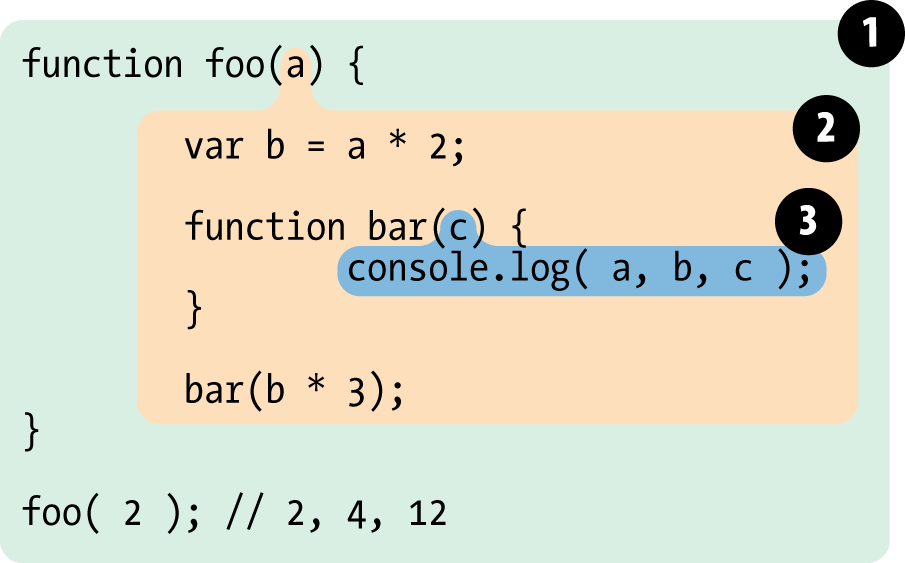
\includegraphics{fig2.png}
\caption{Nested scope \cite{getify}}
\end{figure}

The function \texttt{foo} is defined \emph{in} the global scope (1) (see
next section), and is therefore accessible from all parts of this
program. \texttt{foo} itself defines a new scope (2) which includes the
identifiers \texttt{a}, \texttt{b} and \texttt{bar}. \texttt{bar}
defines a new scope (3) within \texttt{foo}, defining only the
identifier \texttt{c}. As can be seen, the innermost scope (3) has
access to its own identifiers, as well as to the ones defined in its
containing scope (2).

\subsubsection{Scoping Models}\label{scoping-models}

As mentioned above, the rules for when a new scope is defined differ
depending on the programming language. Usually, a language implements
multiple of the following rules.

\begin{description}
\item[Global scope]
Variables that are accessible from \emph{any point} in the program are
in the global scope. The original BASIC programming language only
implemented global scope.
\item[Block scope]
Any logical block, often denoted by containing curly braces (\texttt{\{}
and \texttt{\}}), will create a new scope. This is the case in the C
programming language, amongst others.
\item[Function scope]
Any function definition defines a new scope. Parameters of the function
are part of this newly defined scope, as well as variables and function
defined within that function. JavaScript implements function scope.
\item[Expression scope]
A variable’s scope is limited to a single expression. This useful for
very short-living, temporary variables. It is implemented by many
functional languages, for example Python and ECMAScript 6.
\end{description}

JavaScript, as of ECMAScript 5, implements only global and function
scope\footnote{There are exceptions through the keywords `with` and `except` and the function `eval`.}.

In JavaScript, the run-time environment defines what is in the global
scope. The JavaScript engines in web browsers usually provide access to
the \ac{dom} through the \texttt{document} object, whereas Node.js
provides the \texttt{require} function to include CommonJS-style
modules.

In contrast, the Java programming language implements block scope, but
no global scope. - Functions define a new scope; blocks do not (in
JavaScript)

\subsubsection{Common scoping problems}\label{common-scoping-problems}

The following are common phenomena that arise through scoping and may be
the cause of problems and misconceptions. Though being typical for
JavaScript, many of those problems can arise in other programming
languages, in the same or similar form, as well.

These phenomena can in most cases be either helpful or hindering, and
thus be desired or undesired. The goal of the concept developed in this
thesis is to make the developer recognize those phenomena during
author-time, and thus avoid misconceptions and reduce errors.

\begin{description}
\item[Hoisting]
is the implicit process, as done by the JavaScript engine, of moving
variable and function declarations „from where they appear in the flow
of the code to the top of the code“ \cite{getify}. By code,
\citename{getify} refers to the scope block. Any variable declaration
inside a scope block is hoisted to the top of the scope block.

\begin{verbatim}
        function foo() {
          a = 2;
          var a;
          console.log( a );
        }
\end{verbatim}

The above code is actually processed as:

\begin{verbatim}
        function foo() {
          var a;
          a = 2;
          console.log( a );
        }
\end{verbatim}

The variable declaration of \texttt{a} is moved, or „hoisted“, to the
top of the scope block of \texttt{foo}. Hoisting can impose unexpected
behaviour, especially when declaring variables of the same name in
nested scopes.
\item[Closure]
is a common phenomenon in JavaScript programs, and is widely used,
though being generally seen as hard to understand. Citing
\citename{getify}, closure is „when a function is able to remember and
access its lexical scope even when that function is executing outside
its lexical scope.“ \citeyear{getify} As functions are first-class
objects in JavaScript, they can be passed around like variables, for
example as callbacks. A function can also return another function.
However, JavaScript works with \emph{lexical scope} and, according to
the nesting rules presented before, a function must always have access
to its ancestor scopes. Thus, when a function is being returned or
passed as a callback, an instance of the whole scope chain is returned
or passed along with the function. In other words, the function „closes“
or „forms a closure“ over its ancestor scopes. In most cases, this
behaviour is desired. Anyway it is important to recognize closures, as
they may impact performance: the closed-over scopes have to stay in
memory as long as a reference to the closure exists. Closure may also
lead to unexpected behaviour, for example if a variable defined outside
of a closure is used inside of it (see \citeasnoun*[Ch. 5]{getify} for
examples).
\item[Shadowing]
is a consequence of nested scopes. If a variable (1) is defined in an
ancestor scope, and a new variable (2) of the same name is defined in a
descendant scope, the descendant scope has no access to (1). This is due
to the mechanism of variable lookup explained above. Variable (1) is
said to be \emph{shadowed} by variable (2). As with most of the
phenomenons listed here, this can either be desired or unwanted
behaviour. A good solution to avoid shadowing is choosing different
variable names throughout nested scopes.
\item[Implicit variable declaration]
JavaScript allows for the creation of variables and object properties in
an implicit way (\emph{silently}). Instead of declaring a variable using
a \texttt{var} statement, they can as well just be used without prior
declaration, for example like this:

\begin{verbatim}
i = 3;
\end{verbatim}

Variables used without prior declaration are implicitly declared in the
\emph{global
scope}\footnote{ECMAScript 5’s \emph{strict mode} considers this an error.}.
As this is usually unwanted behaviour, it is considered good practice to
always declare variables explicitly. However, this problem is already
addressed by linters (see \fullref{similar}).
\item[Lookup performance]
The variable lookup through scope chains, as described above, can have
an impact on the performance of an application. Each time a variable is
encountered, the JavaScript engine performs the lookup process,
navigating from the bottom of the scope chain upwards until it is found.
If a variable, which is defined in an ancestor scope (the global scope,
for example), is accessed within a deeply nested scope, the lookup
process slows down the execution of the program, as shown by
\citeasnoun{castorina}. He furthermore suggests to cache the variable in
a „closer“ scope, if possible.
\end{description}
